\documentclass[10pt]{article}
\usepackage[a4paper,margin=17mm]{geometry}
\usepackage{amsmath,amssymb,graphicx,hyperref}
\hypersetup{colorlinks=true,urlcolor=blue}
\setlength{\parindent}{0pt}\setlength{\parskip}{5pt}
\begin{document}
\begin{center}\Large Complete public-target composition\\[3pt]
\normalsize Rust interface and signed raw-index rows, 16 November 2026\\
PCC-20261116-4679b0; signed standing unverified\end{center}
The public compiler joins six distinct raw members to a Curve25519 target
with complete extended Edwards addition. Checked roots decode to signed
raw columns $(j,t)$, independently replayed by native Montgomery addition.
Compilation receives no planted labels, signs, scalar or point witnesses.
[pcc:unverified]
\begin{center}\begin{tabular}{lrrrr}
Interface & Variables & Equations & Terms & Degree\\\hline
One cofactor image (v1) &159&161&483&2\\
Six members, target and distinct indices &1059&1089&3323&2
\end{tabular}\end{center}
These are counts for different outputs/arities, not runtime or attack work.
\begin{center}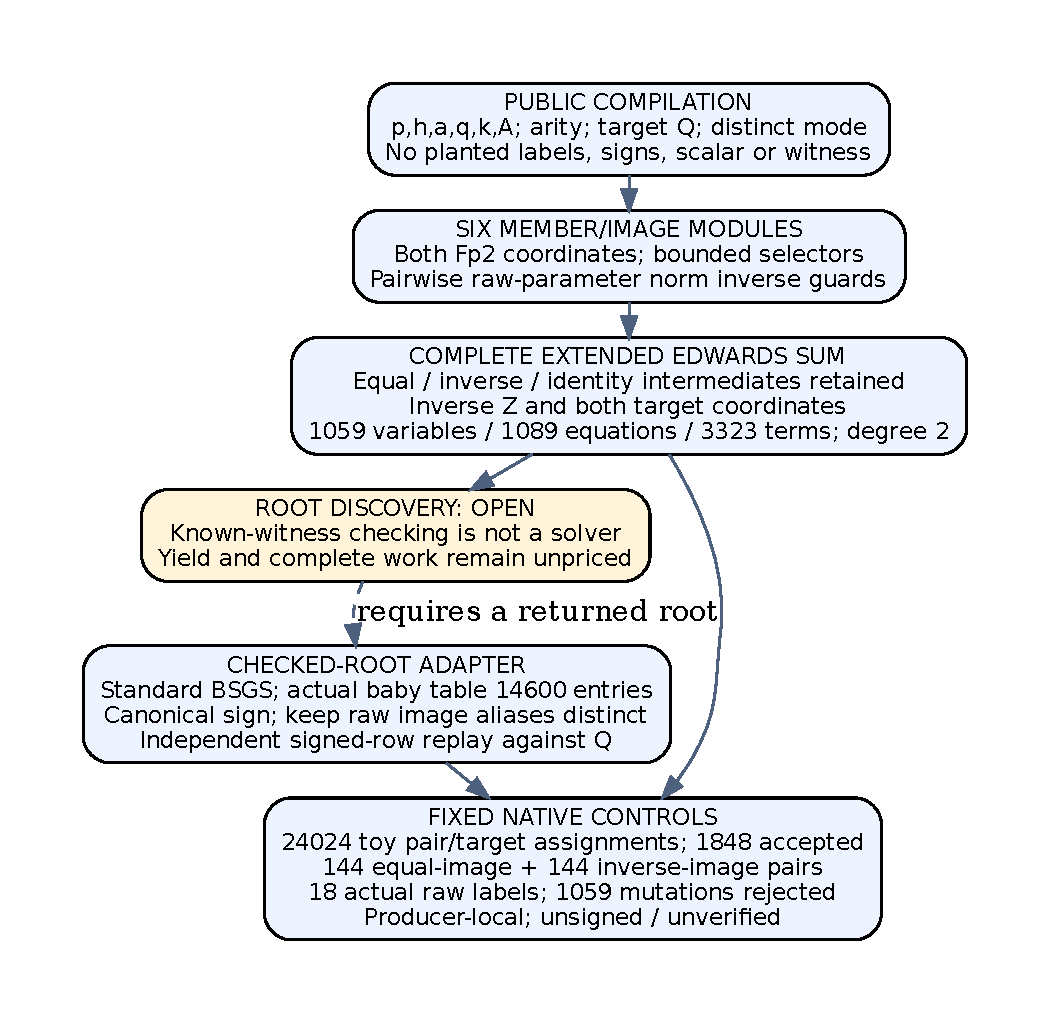
\includegraphics[width=0.98\linewidth,height=132mm,keepaspectratio]{pipeline.pdf}\end{center}
\textbf{Actual instance.} $p=2^{255}-19$, $A=486662$, $a=60824497$,
$q=213156431$, $k=20633$. Earlier exact-order contracts give $B=kq$
raw columns. Point-image aliases remain separate columns; identity leaves
are explicitly excluded. Prime-field/order/map and odd-order image-group
contracts remain external; no new compiler theorem is supplied.
\newpage
\begin{center}\Large Domain, controls and next gate\end{center}
\textbf{Intended conditional semantics.} Copy member equations with
explicit variable offsets. In distinct mode, guard every $N(z_i-z_j)$ by
an inverse; nonsquare two makes this reject equal parameters without
rejecting point aliases. Convert nonidentity odd-order images by
\[
x=Cu/v,\quad y=(u-1)/(u+1),\quad C^2=-(A+2),\quad d=-(A-2)/(A+2).
\]
Guard $v,u+1$, then use RFC8032 section5.1.4's complete eight-product
formulas. Retain $XY=ZT$, $-X^2+Y^2=Z^2+dT^2$, inverse $Z$ and both
target equations $X=x_QZ$, $Y=y_QZ$. Identity is $(0,1)$. Numerical
conversion/nonsquare conditions are checked, not primality, point count or
exact order. Finite controls do not prove compiler soundness/completeness.

\textbf{Raw rows.} Decode $j,z$, recover $t$ from
$z/h^j=(h^a)^t$ by HAC Algorithm3.56, bound $t<q$ and replay its power.
Actual table:14600 babies; hard cap:$2^{20}$. Independently recompute
canonical sign and replay the signed row, combining only equal raw labels.
This computes no elliptic scalar log. For $O(B)$ successful fixed-arity
rows, standard BSGS costs soft-$O(B\sqrt q)$ work and $O(\sqrt q)$ space,
separately charged from root discovery and failures.

\textbf{Actual controls.} All 18 fixed signed leaves recover original
labels. Five aggregate cases cover cancellation, doubling, identity
intermediates and six distinct parameters. Equations and independent row
replay agree. All 1059 variable increments reject; wrong target, repeated
parameter, malformed shapes and memory/arity caps reject. [pcc:unverified]

\textbf{Toy population.} Fixed $p=101,A=95,C=2,d=99,h=(17,12),a=17,q=3,k=8$:
104 curve points and13 eightfold images by full affine enumeration. Of 24
raw columns, $(1,2),(8,2)$ have identity images and remain explicitly
recorded as exclusions;44 signed leaves remain. All 1848 distinct-raw
ordered pairs against13 targets give 24024 canonical assignments,1848
accepted and zero disagreement with native addition. There are 144
equal-image pairs,144 inverse-image pairs and144 identity sums. This does
not exhaust arbitrary auxiliary assignments. [pcc:unverified]

\textbf{Reproduction/failures.} First build:unused private Clone derive
and extra Poly borrow; exact source/log retained. Corrected release suite:
two tests pass; fmt/strict all-target Clippy pass. A 55368-byte archive
preserves 43 inputs; ten compiled-in hashes match. Pre-call qualifier,
compressed full system, first witness and entire toy trace are retained.
Earlier v1 archives/direct Lean bindings stay unchanged. These are local
controls, not signed execution.

\textbf{Next gate.} Discover original roots from public inputs under a
bounded frozen solver protocol; charge setup, failures, indexing, selection
and recovery under unchanged route criteria. Quadratic degree/sparsity
supplies no gamma/yield theorem. No new solver campaign, sampling,
benchmark, paid job or broad library rerun occurred.

\textbf{Sources.} Source-linked REPORT.md;
\href{https://www.rfc-editor.org/rfc/rfc8032\#section-5.1.4}{RFC8032 sec. 5.1.4};
\href{https://www.rfc-editor.org/rfc/rfc7748\#section-4.1}{RFC7748 sec. 4.1};
\href{https://cacr.uwaterloo.ca/hac/about/chap3.pdf}{HAC sec. 3.6.2};
\\Frozen member, coset and reduction records; native APIs. KB unavailable;
primary-source fallback. No novelty claim for established methods.
\end{document}
